\documentclass{article}
\usepackage[utf8]{inputenc}
\usepackage[margin=1in,includefoot]{geometry}
\usepackage{graphicx}
\usepackage{subcaption}
\usepackage{enumerate}
\usepackage{xfrac}
\usepackage{url}
\usepackage{amsmath}
\usepackage{mathtools}
\usepackage{blindtext}
\usepackage[numbers,sort&compress]{natbib}
\usepackage{listings}
\usepackage{color}
\usepackage{filecontents}
\usepackage{natbib}
\usepackage{bibentry}
\nobibliography*
\lstset{language=Matlab,
basicstyle=\ttfamily,
keywordstyle=\color{blue}\ttfamily,
stringstyle=\color{red}\ttfamily,
commentstyle=\color{green}\ttfamily,
morecomment=[l][\color{magenta}]{\#}
}
\usepackage{multicol}
\begin{filecontents}{mytestbib.bib}
@book{goossens93,
    author = "Cambridge University Department of Engineering",
    title = "3G1 Laboratory: Investigating the lac Operon",
    year = "2017",
    publisher = "University of Cambridge",
}
@book{permease,
    author = "Crandall, M; Koch, A.L",
    title = "Temperature-Sensitive Mutants of Escherichia Coli Affecting Beta-Galactoside Transport",
    year = "1971",
    publisher = "Journal of Bacteriology. 105 (2): 609-19",
}
@book{miller,
    author = "Miller JH",
    title = "A Short Course In Bacterial Genetics: A Laboratory Manual And Handbook For Escherichia Coli And Related Bacteria",
    year = "1992",
    publisher = "Trends in Biochemical Sciences-Library Compendium, 18:193",
}
\end{filecontents}

\begin{document}
\begin{titlepage}
	\begin{center}
	\line(1,0){450}\\
	[0.25in]
	\huge{\bfseries 3G1 Investigating the lac Operon} \\
	[0.25in]
     \large Investigation on the feedback system of the lac Operon under different conditions\\
     \line(1,0){450} \\
	[12cm]
	\textsc{\Large Xiaoding Lu \\[1cm] xl402 \\ Pembroke College \\[1.2cm] 02.11.2018}\\
	\end{center}
	\begin{flushright}

	\begin{figure}[htp]
	\begin{flushright}
	\end{flushright}
	\end{figure}
	\end{flushright}

\vspace{2cm}

\end{titlepage}

\cleardoublepage
\pagenumbering{roman}
\cleardoublepage
\pagenumbering{arabic}
\section{Introduction}
The lactose operon (lac operon) in \textit{Escherichia coli} is one of the first and most studied examples of gene regulation and control in prokaroyotes. The lac operon regulates the production of enzymes involved in the metabolism of lactose and incorporates both positive and negative feedback in its regulatory network \cite{goossens93}. \\ \\
Figure \ref{fig:lac_operon} shows the simplified schematic for a lac operon. It is known that lacZ codes for $\beta$-glactosidase which is the protein which breaks down lactose, lacY codes for galactoside permease (refered to as permease) which are membrane transport proteins which increases the uptake of of $\beta$-glactosides using hydrogen, sodium or lithium ions in the cotransport \cite{permease}, lacA codes for transacetylase which participates in the reaction which breaks down lactose. lacl codes for the repressor protein, which binds onto the promoter site ($P$) inhibiting gene expression. \\ \\
The aim of this experiment is to assay the activity of $\beta$-glactosidase under different conditions in order to illustrate gene control as predicted by simple models of this system.
\begin{figure}[htp]
	\centering
	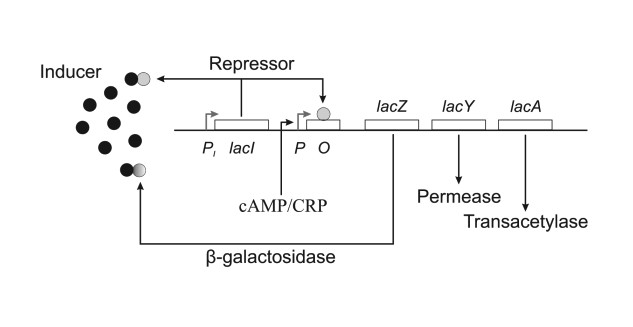
\includegraphics[width=0.8\linewidth]{lac.png}
	\caption{The lac operon schematic}
	\label{fig:lac_operon}
\end{figure}

\section{Methodology}
Two expirements are carried out with detailed procedures explained in the handout \cite{goossens93}. Experiment 1 uses the $\Delta lacl$ strain of the bacteria (with lacl gene turned off), different inducers such as lactose, IPTG, glucose (and control) are used to investigate the behaviour of the lac operon without the repressor. \\ \\
In the second experiment, three different strains of bacteria (wild type, $\Delta lacY$ and $\Delta lacIZY$) are investigated under different inducers (IPTG and lactose), the activity of $\beta$-glactosidase is measured at constant intervals (60 minutes to 150 minutes with 30 minutes intervals). \\ \\
The activity of $\beta$-glactosidase is quantified using the o-nitrophenyl-$\beta$-$D$-glactoside (ONPG) assay as described by Miller \cite{miller}. $OD_{600}$ is taken first to measure the bacterial cell density in the culture. The sample is then mixed was Z-buffer, SDS and chloroform, then vortexed for 10 seconds to lyse the cells. ONPG is then added and samples are incubated at 37 degrees celcius for 20 minutes. $Na_2CO_3$ is then added to stop the reaction. All the samples are then left until the end when $OD_{420}$ and $OD_{550}$ readings are taken. $OD_{420}$ measures of the amount of o-nitrophenol which is the product of $\beta$-galactosidase catalyzed breakdown of ONPG thus it is a measure of $\beta$-galactosidase activity, $OD_{550}$ is measured to correct for cell debris. Finally $\beta$-glactosidase activity ($\beta A$) is calculated using the following equation (with the constant 1000 with unit mol/cell$\times$min$\times$ml which converts the activity per time, per volume, per cell density to molecules of enzyme per cell):
$$
\beta A = 1000 \dfrac{OD_{420}-1.75OD_{550}}{t\times V\times OD_{600}}
$$
In the equation above, $t$ is the incubation time for the assay in minutes (20 mins in this case), and $V$ is the volume in ml of the culture used in the assay (in this case, 0.2ml).
\section{Discussion of Feedback Mechanisims}
In the wild type (wt) lac operon, there are four feedback mechanisims, two positive and two negative. The two positive feedbacks are:
\begin{enumerate}
  \item Active transport by lactose permease producing a higher concentration of $\beta$-galactosides and lactose inside the cell thereby increasing the expression of lacY which codes for lactose permease
  \item Transgalactosylation by $\beta$-galactosidase produces allolactose from lactose thereby increasing the expression of lacZ which codes for $\beta$-galactosidase
\end{enumerate}
The two negative feedbacks are:
\begin{enumerate}
  \item $\beta$-galactosidase hydrolyses allolactose thereby decreasing the amount of inducer in the cell which reduces the amount of $\beta$-galactosidase
  \item $\beta$-galactosidase hydrolysis of lactose and allolactose also increases the glucose concentration in the cell which causes catabolite repression, making the transcription of lac genes more difficult. This mechanism is bypassed if IPTG is used instead of lactose.
\end{enumerate}
In experiment 1, with the $\Delta lacl$ strain of the bacteria, without the repressor, $\beta$-galactosidase, permease and transacetylase are all constantly expressed, therefore there is no effects of positive feedback since transcription occurs at a constant rate. However the second type of negative feedback persists as the cyclic adenosine monophosphate (cAMP) site is still active and can still influence the binding difficulty of RNA polymerase.\\
In experiment 2, $\Delta lacY$ means no lactose permease is expressed which eliminates the first positive feedback mechanism; $\Delta laclZY$ elinimates all the feedback mechanisims.
\section{Analysis of Results}

\bibliographystyle{plainnat}
\bibliography{mytestbib}
\end{document}
